
\section{Decoding}


\frame{
	\frametitle{Decoding}
	
	In SMT, decoding typically means the Viterbi approximation
	$$\mdd\ustar = \argmax_\mdd f(\mdd)$$ \pause
	
	If the statistical model $f(\mdd)$ does not violate the independence assumptions of the model of translational equivalences 
	\begin{itemize}
		\item steps in a derivation are weighted independently
	\end{itemize}
	
	\pause 
	
	there is a straightforward (tractable) decomposition of $f(\mdd)$ 
	\begin{itemize}
		\item wFSA (phrase-based MT)
		\item wCFG (hierarchical MT)
	\end{itemize}

}

\frame{
	\frametitle{Inside}
	
	The \textsc{Inside} recursion can be generalised to an arbitrary semiring
	
	\[
	\beta(v) = 
	\begin{cases}
		 \bar{1} & \text{if } BS(v) = \emptyset\\
		 {\displaystyle \bigoplus_{e \in BS(v)}} w(e) {\displaystyle\bigotimes_{u \in \tail(e)}} \beta(u) & \text{otherwise}
	\end{cases}
	\] \pause
	
	\begin{itemize}
		\item efficient bottom-up dynamic program $O(|G|)$\\
		$|G|$ is the size of the graphical representation of $f(\mdd)$
		\begin{itemize}
			\item a lattice (phrase-based MT)
			\item a forest (hierarchical MT)
		\end{itemize}
	\end{itemize}
	
}

\frame{
	\frametitle{Inference}
	
	Viterbi derivation
	\begin{enumerate}
		\item start from the goal (root) 
		\item recursively rewrite every symbol $v$ by solving
		$$e = \argmax_{e \in BS(v)} w(e)\bigotimes_{u \in \tail(e)} \beta(u)$$
	\end{enumerate}
	
	\pause
	Sampling
	\begin{enumerate}
		\item start from the goal (root)
		\item recursively rewrite every symbol $v$ by solving
		$$e \sim p(e \in BS(v)|v) = \frac{w(e)\bigotimes_{u \in \tail(e)} \beta(u)}{\beta(v)}$$
	\end{enumerate}
}

\frame{
	\frametitle{Viterbi}
	
	\only<1>{
	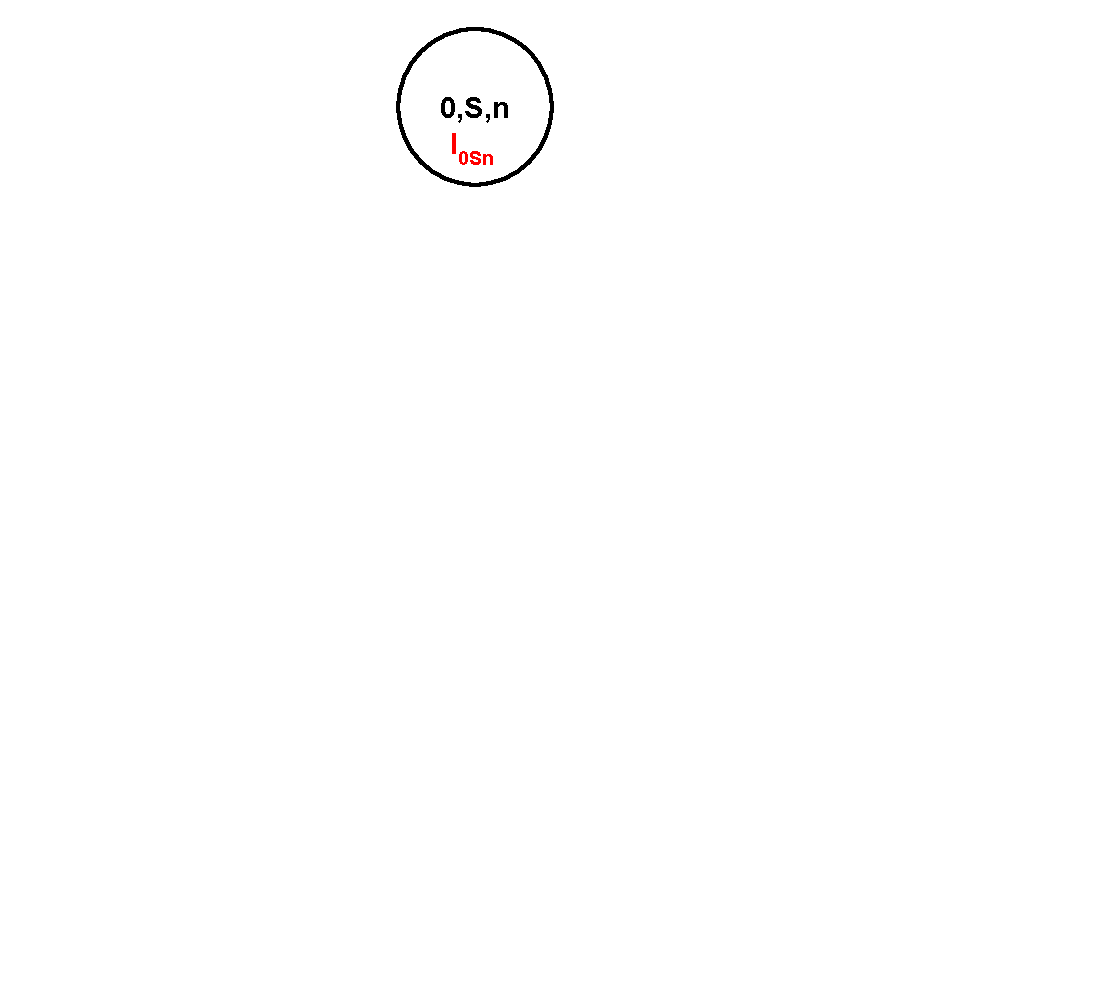
\includegraphics[scale=0.3]{img/viterbi0}
	}
	\only<2>{
	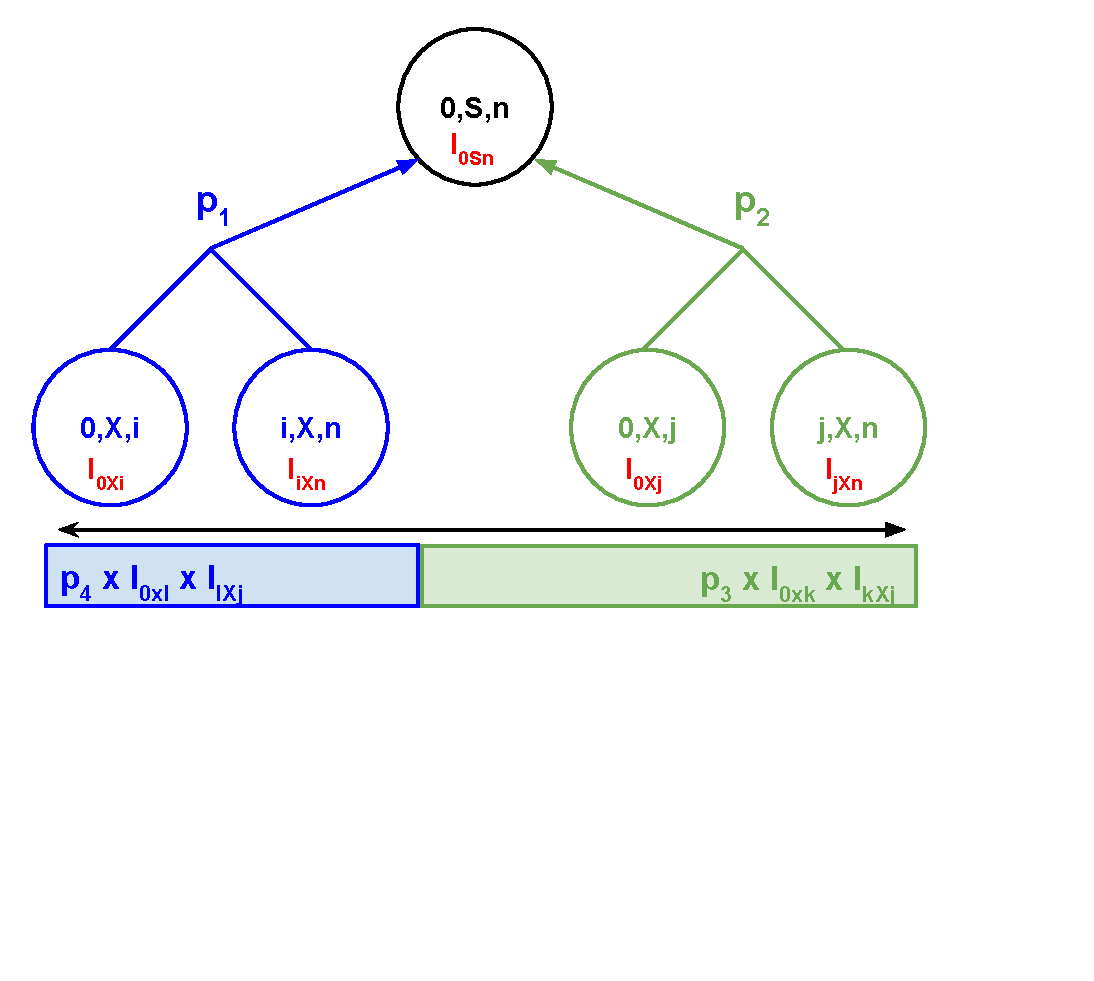
\includegraphics[scale=0.3]{img/viterbi1}
	}
	\only<3>{
	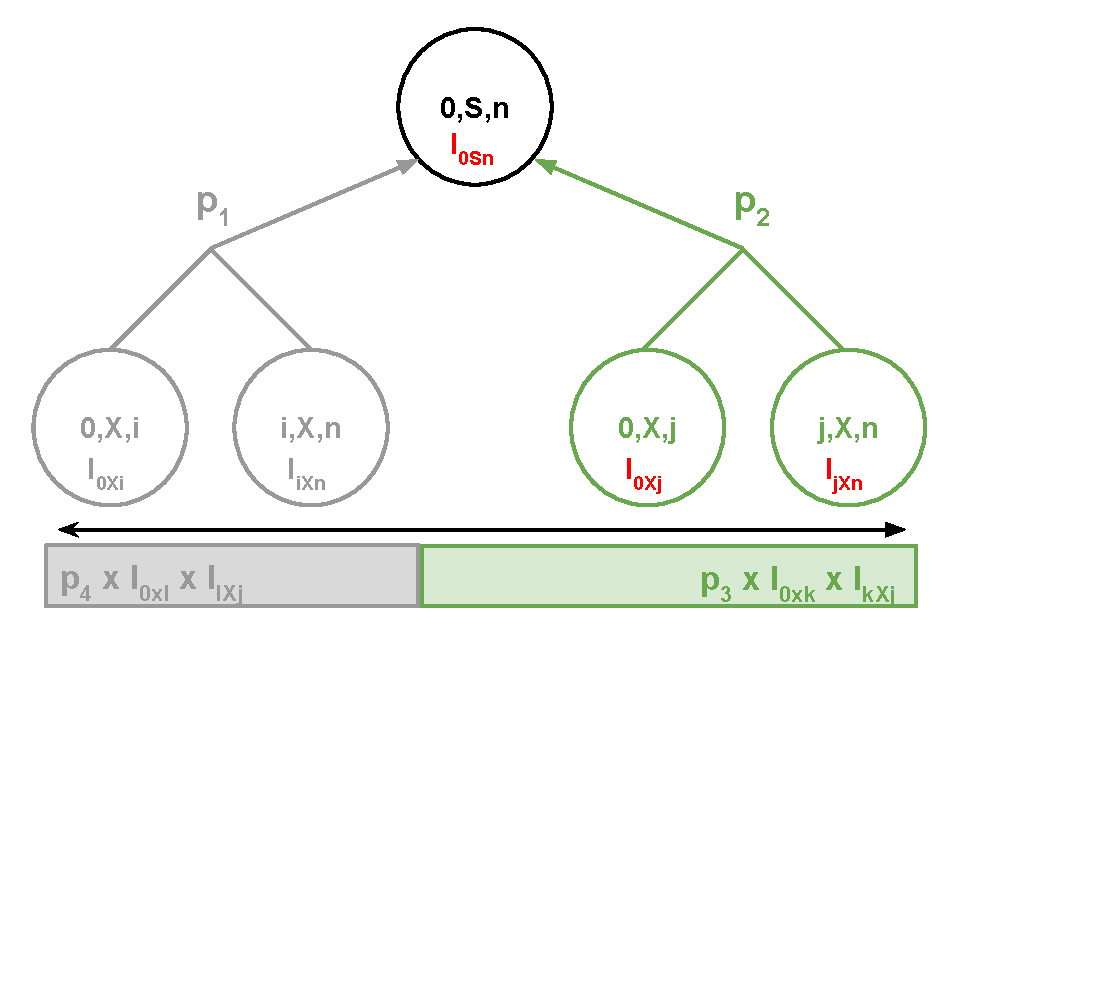
\includegraphics[scale=0.3]{img/viterbi2}
	}
	\only<4>{
	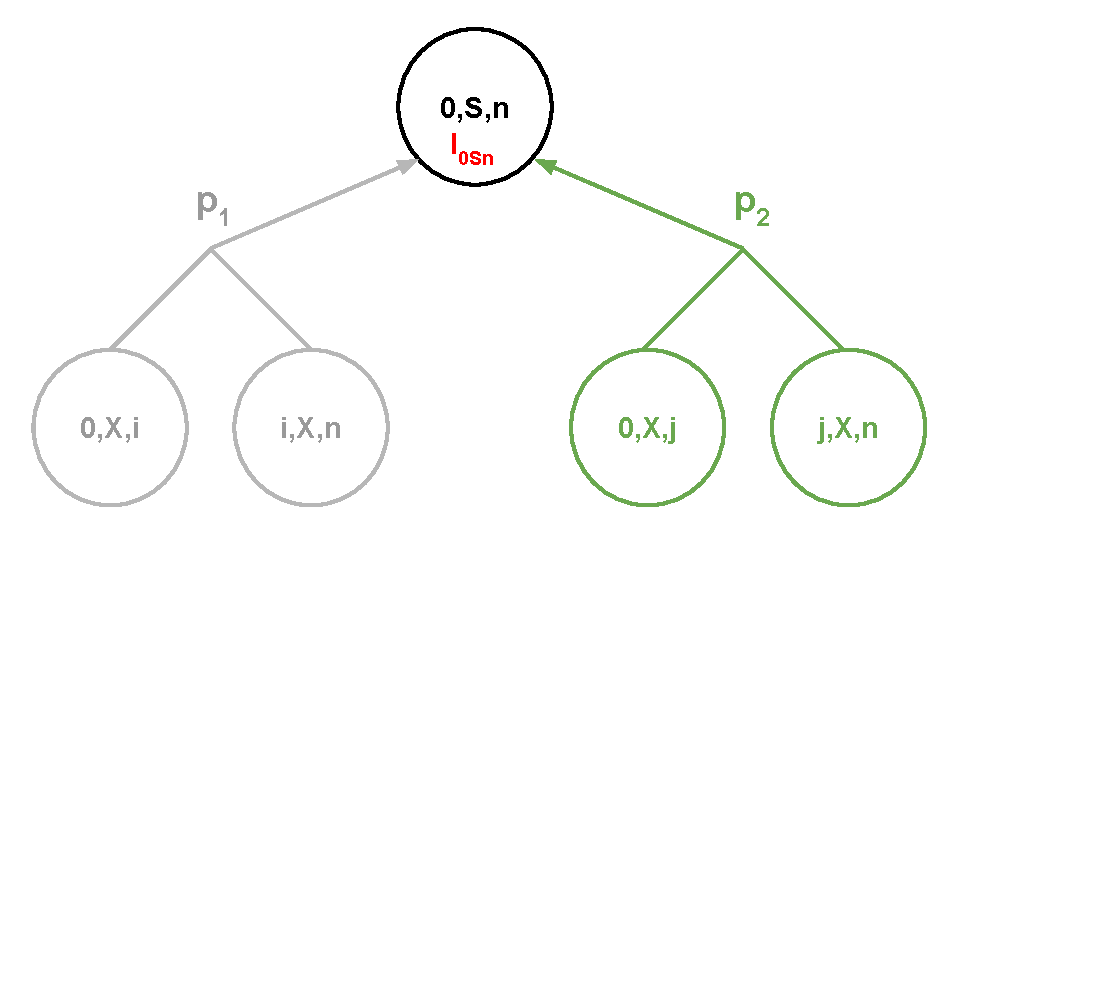
\includegraphics[scale=0.3]{img/viterbi3}
	}
	\only<5>{
	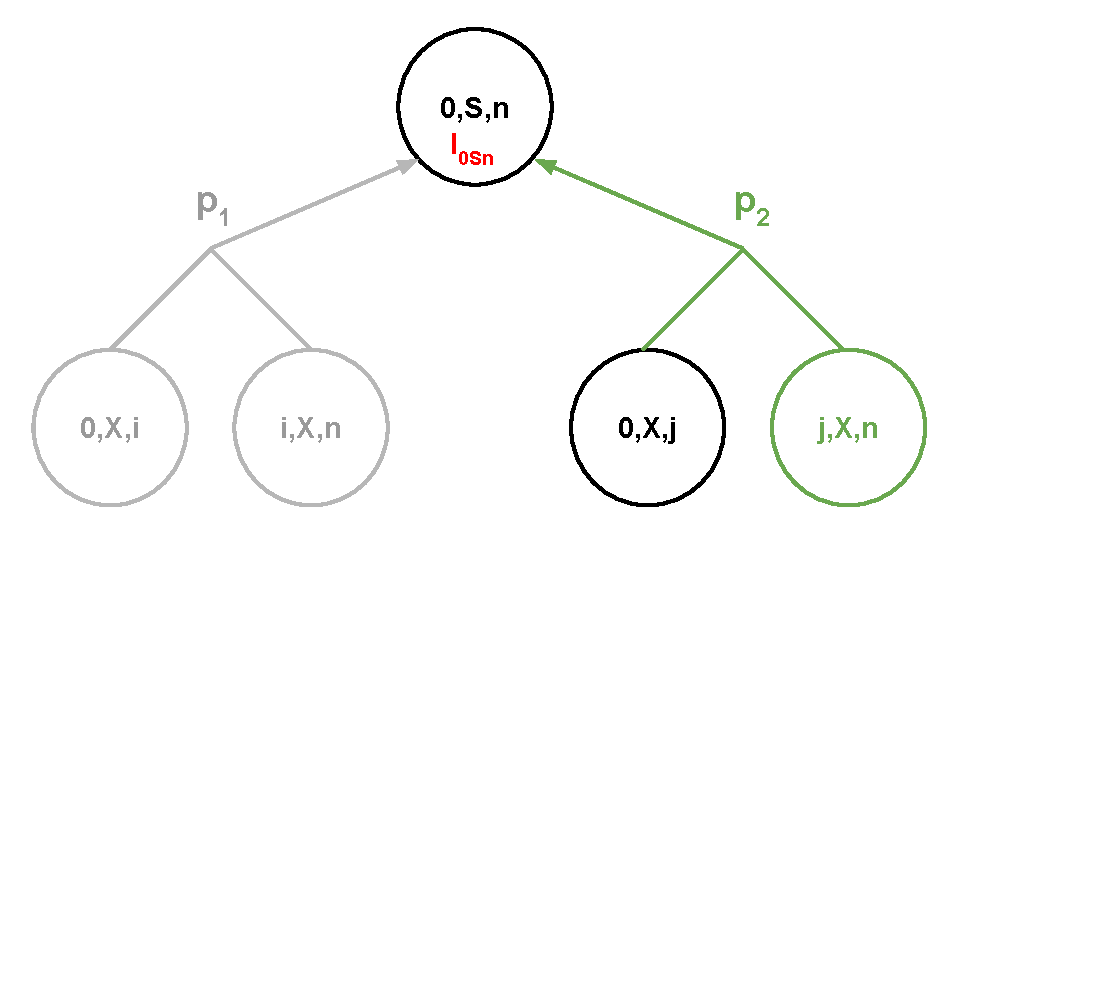
\includegraphics[scale=0.3]{img/viterbi4}
	}
	\only<6>{
	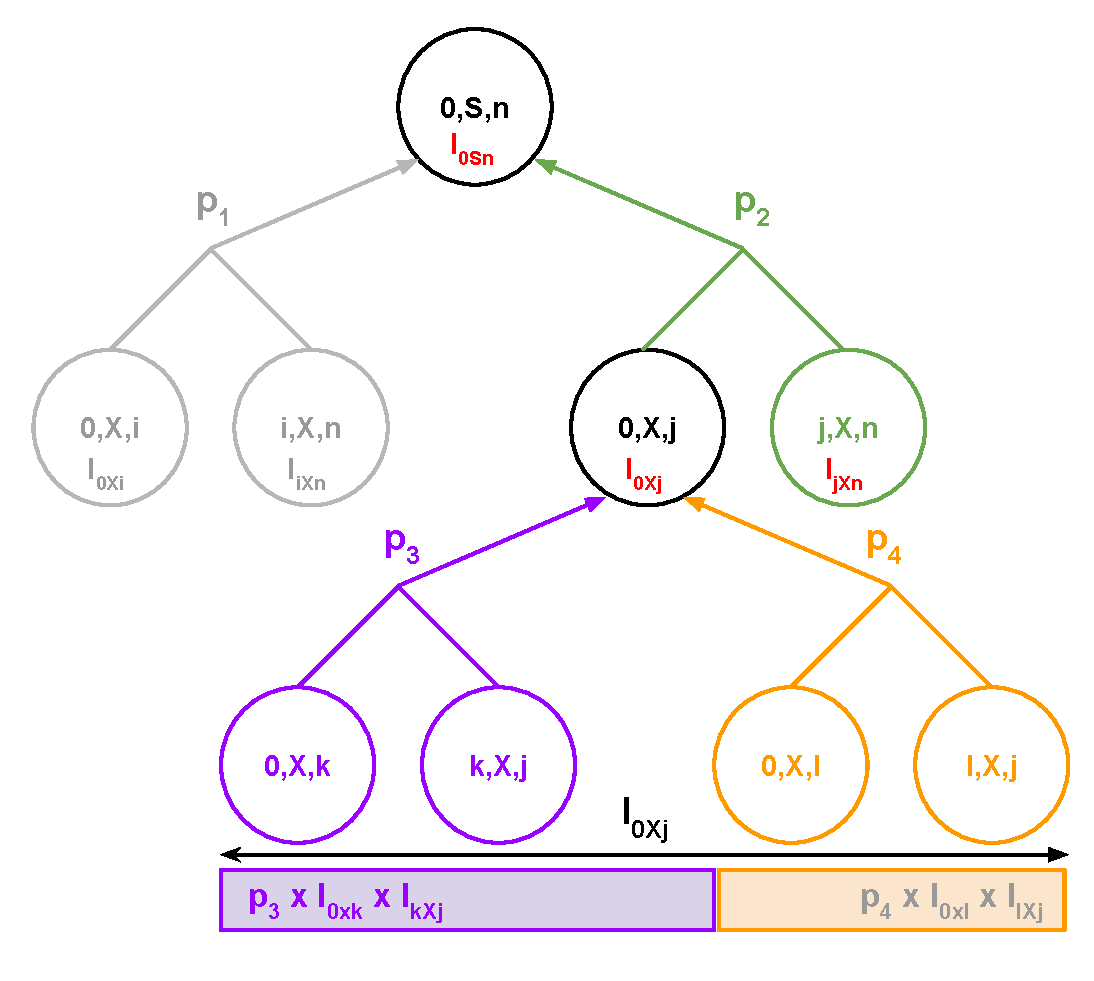
\includegraphics[scale=0.3]{img/viterbi5}
	}
	\only<7>{
	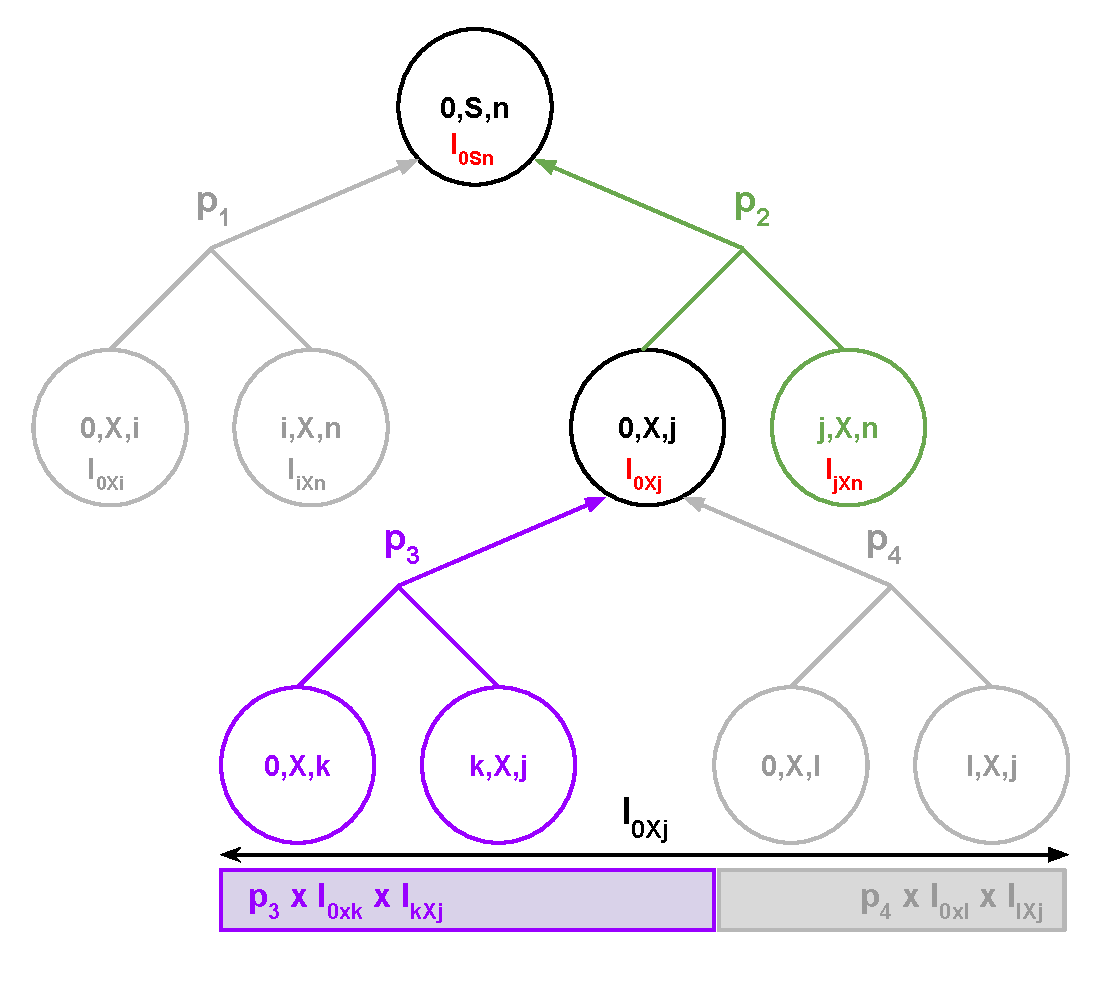
\includegraphics[scale=0.3]{img/viterbi6}
	}
}

\frame{
	\frametitle{Sampling}
	\only<1>{
	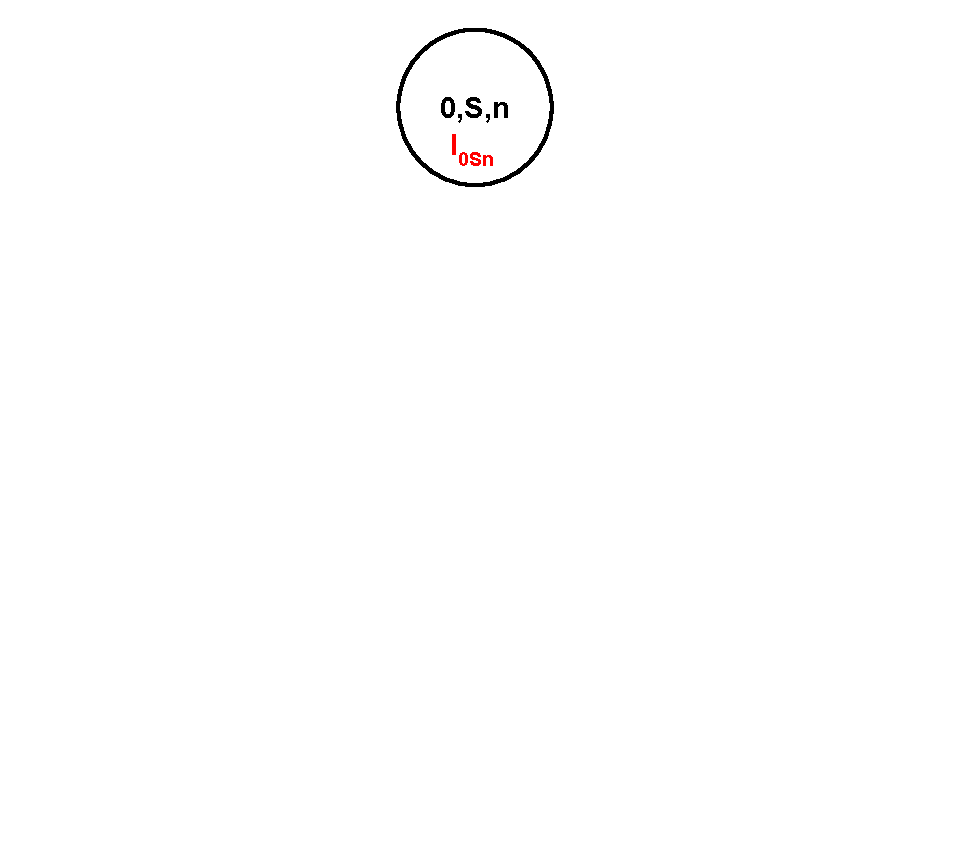
\includegraphics[scale=0.3]{img/sampling0}
	}
	\only<2>{
	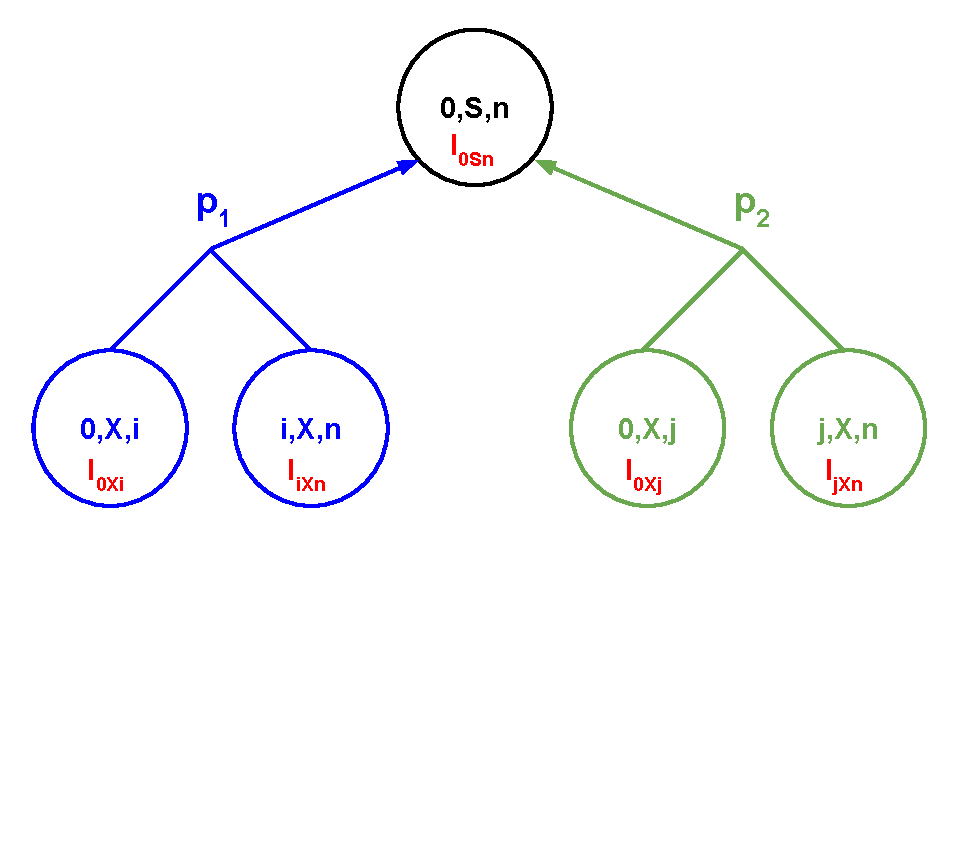
\includegraphics[scale=0.3]{img/sampling1}
	}
	\only<3>{
	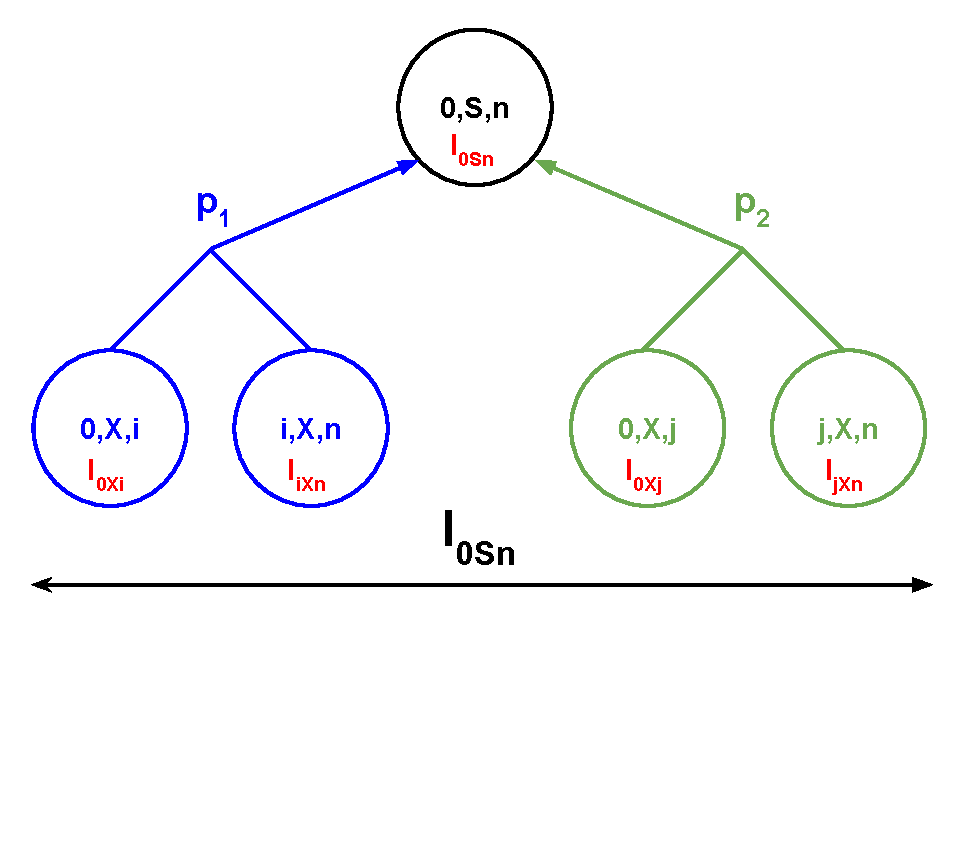
\includegraphics[scale=0.3]{img/sampling2}
	}
	\only<4>{
	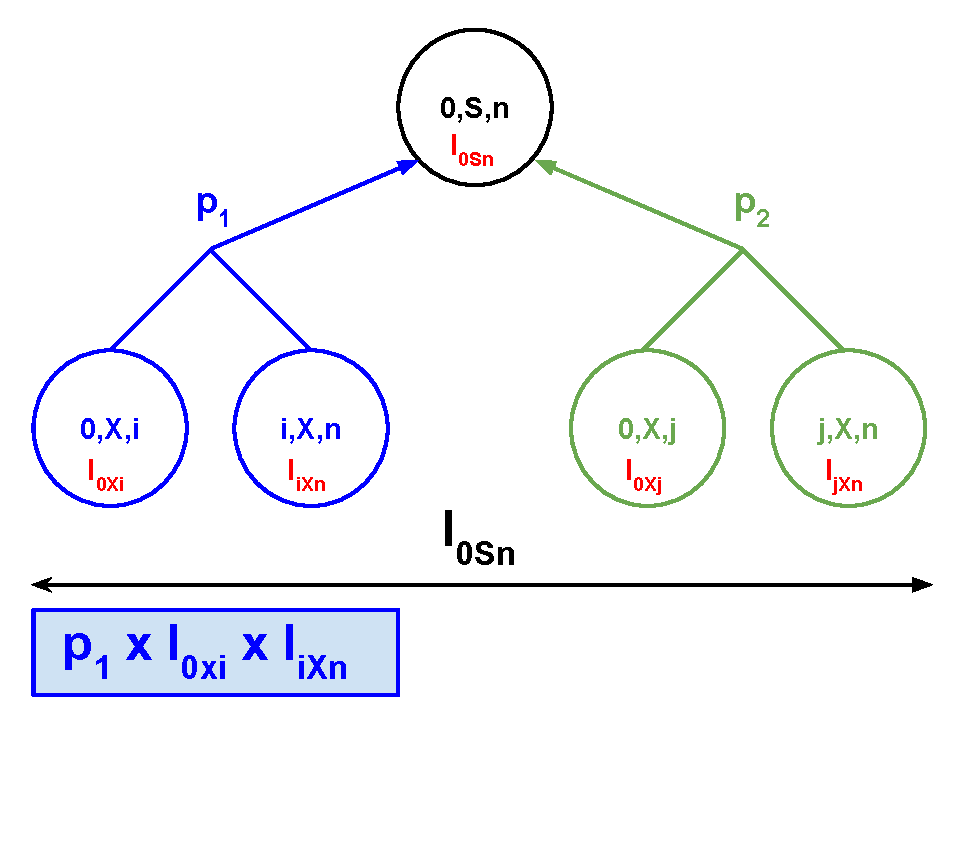
\includegraphics[scale=0.3]{img/sampling3}
	}
	\only<5>{
	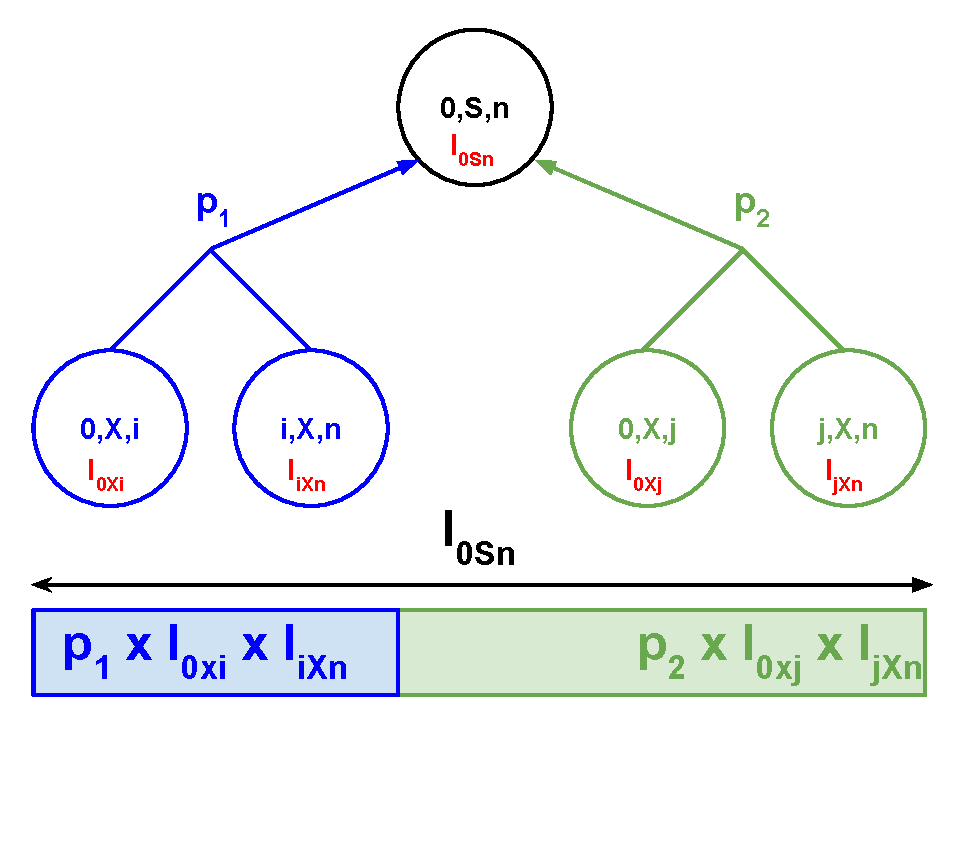
\includegraphics[scale=0.3]{img/sampling4}
	}
	\only<6>{
	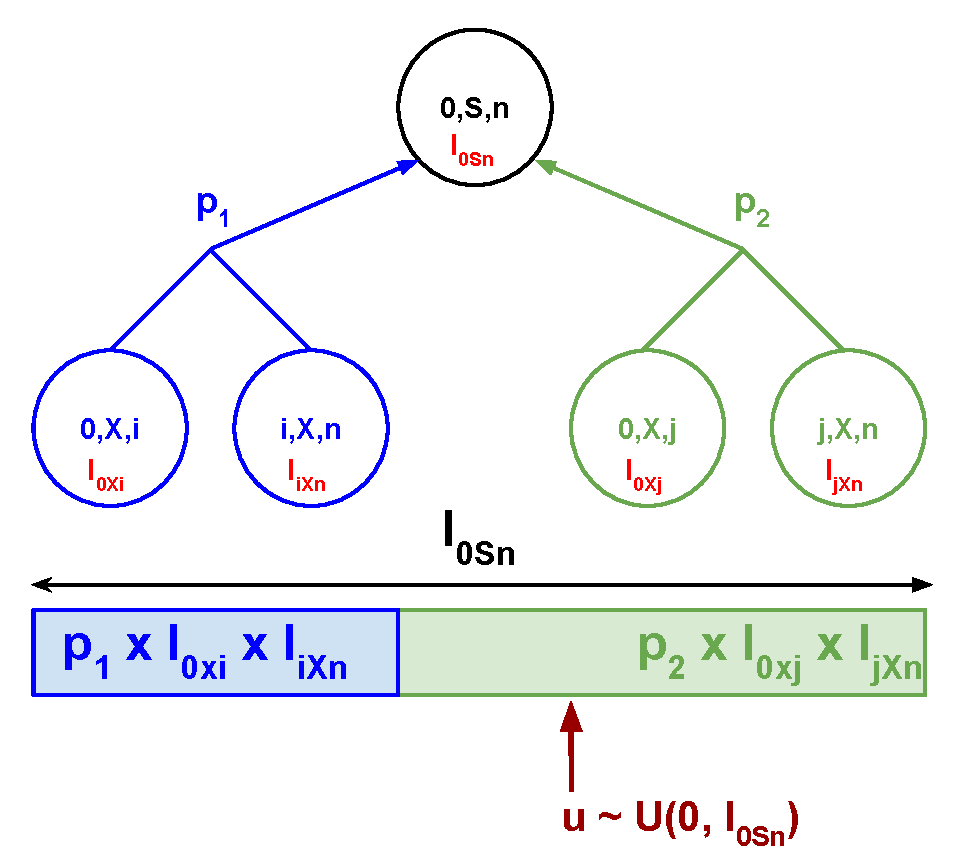
\includegraphics[scale=0.3]{img/sampling5}
	}
	\only<7>{
	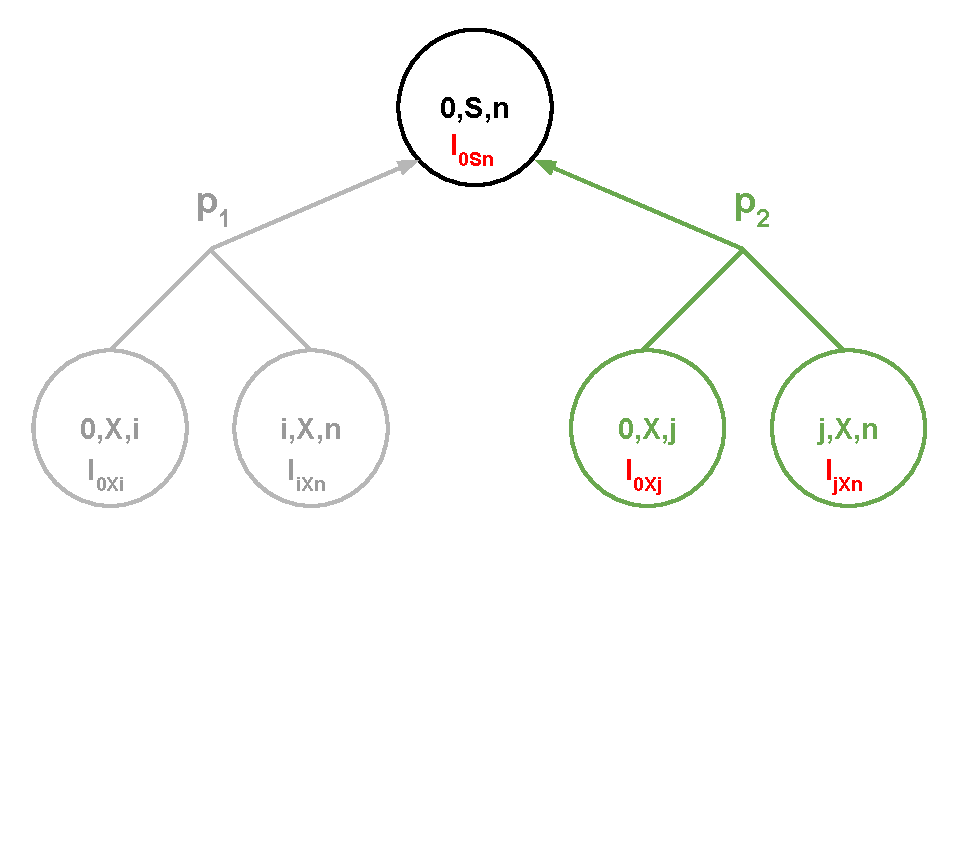
\includegraphics[scale=0.3]{img/sampling6}
	}
	\only<8>{
	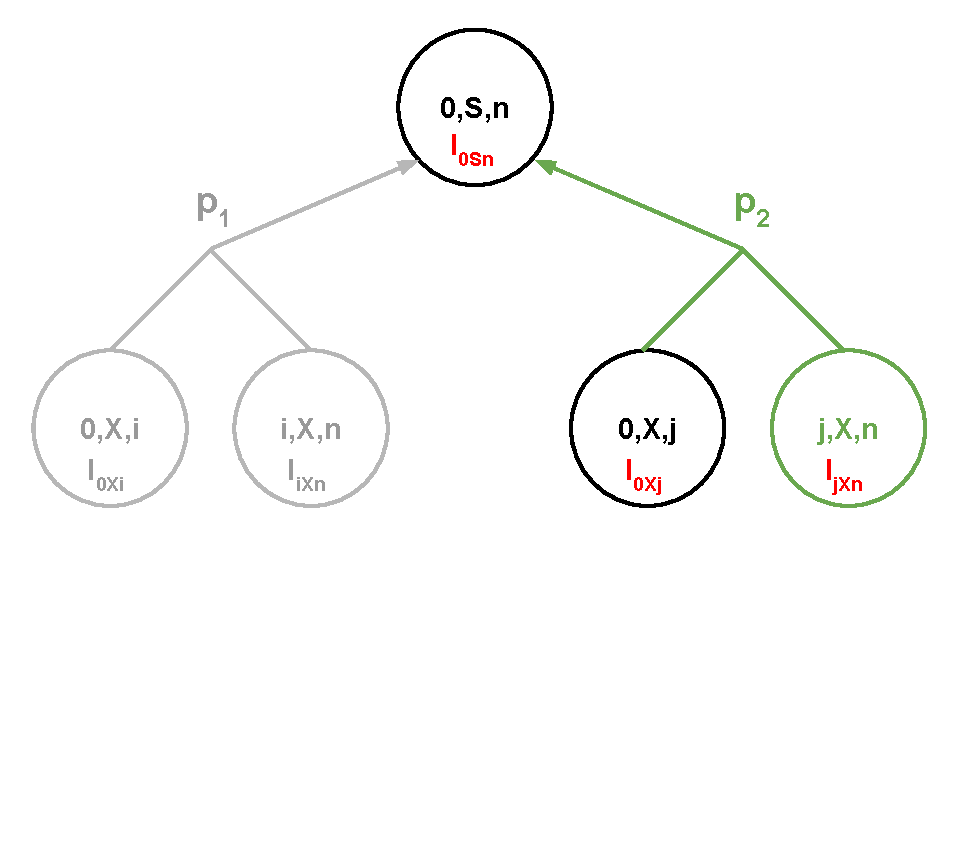
\includegraphics[scale=0.3]{img/sampling7}
	}
	\only<9>{
	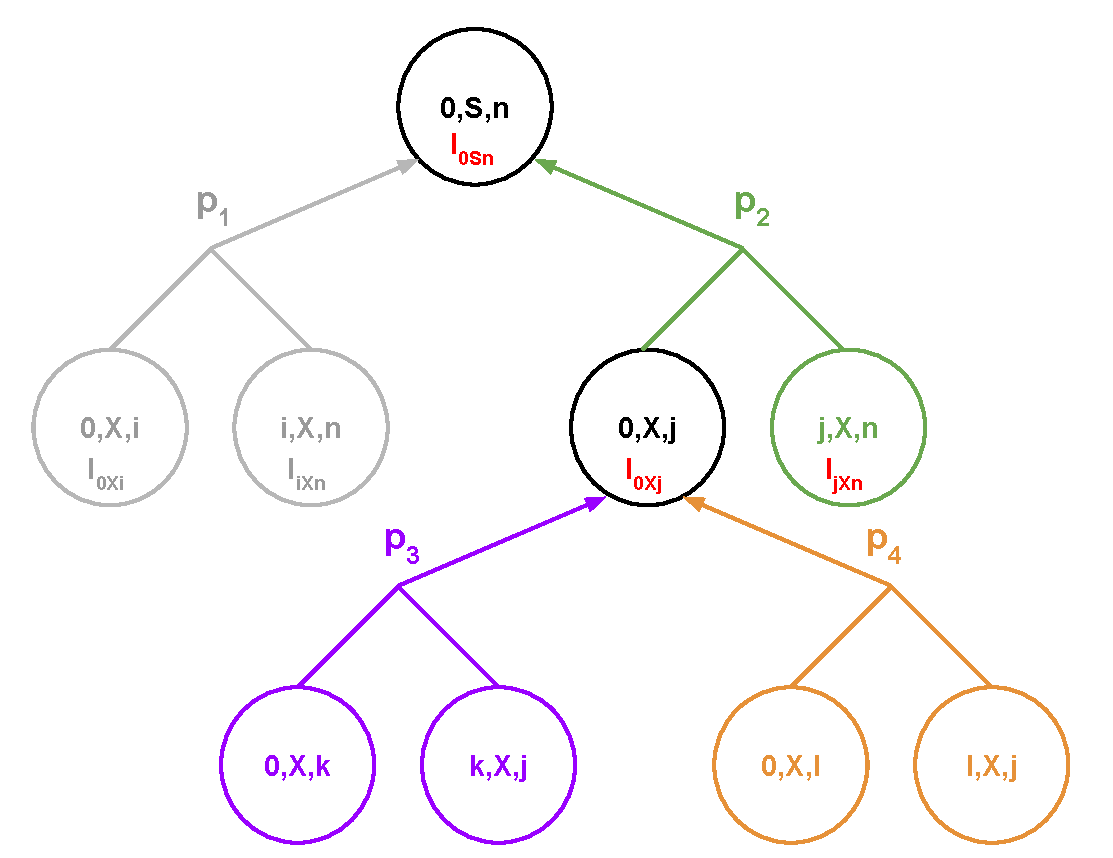
\includegraphics[scale=0.3]{img/sampling8}
	}
	\only<10>{
	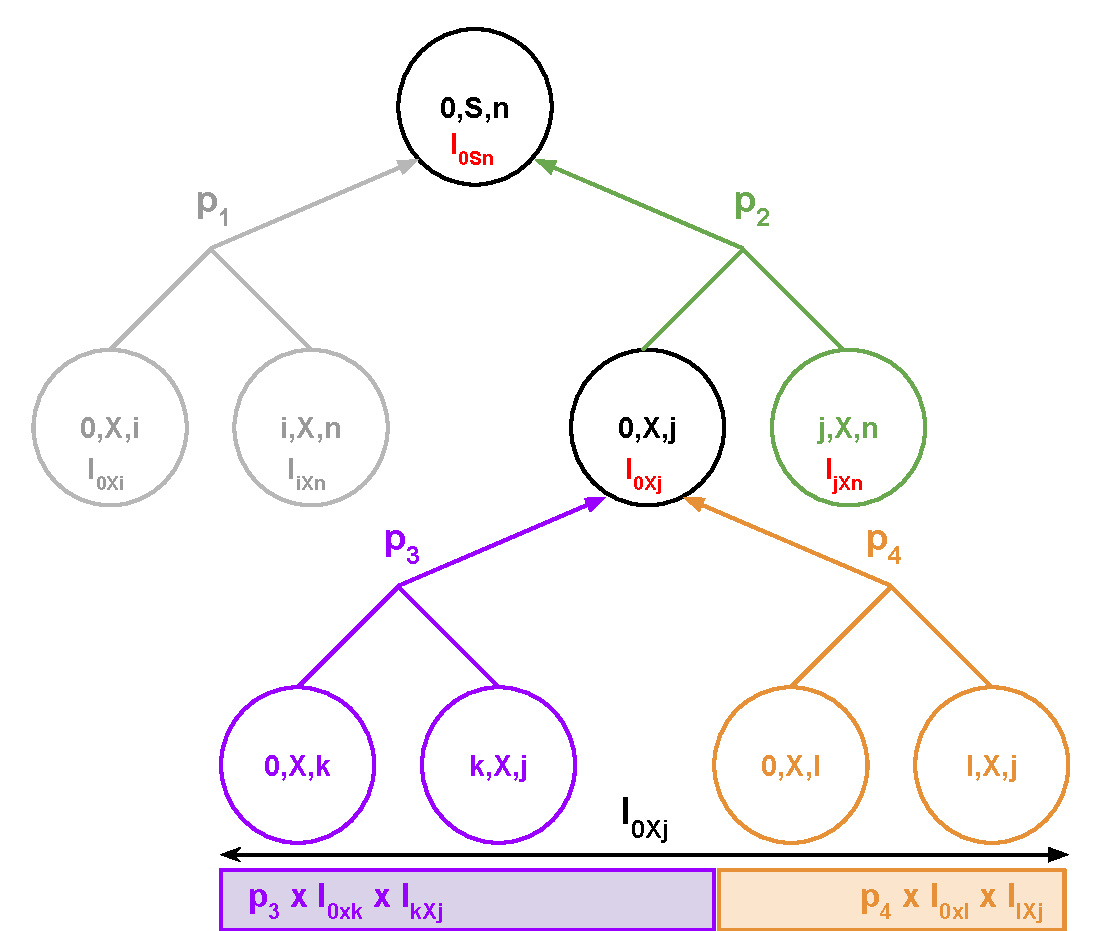
\includegraphics[scale=0.3]{img/sampling9}
	}
	\only<11>{
	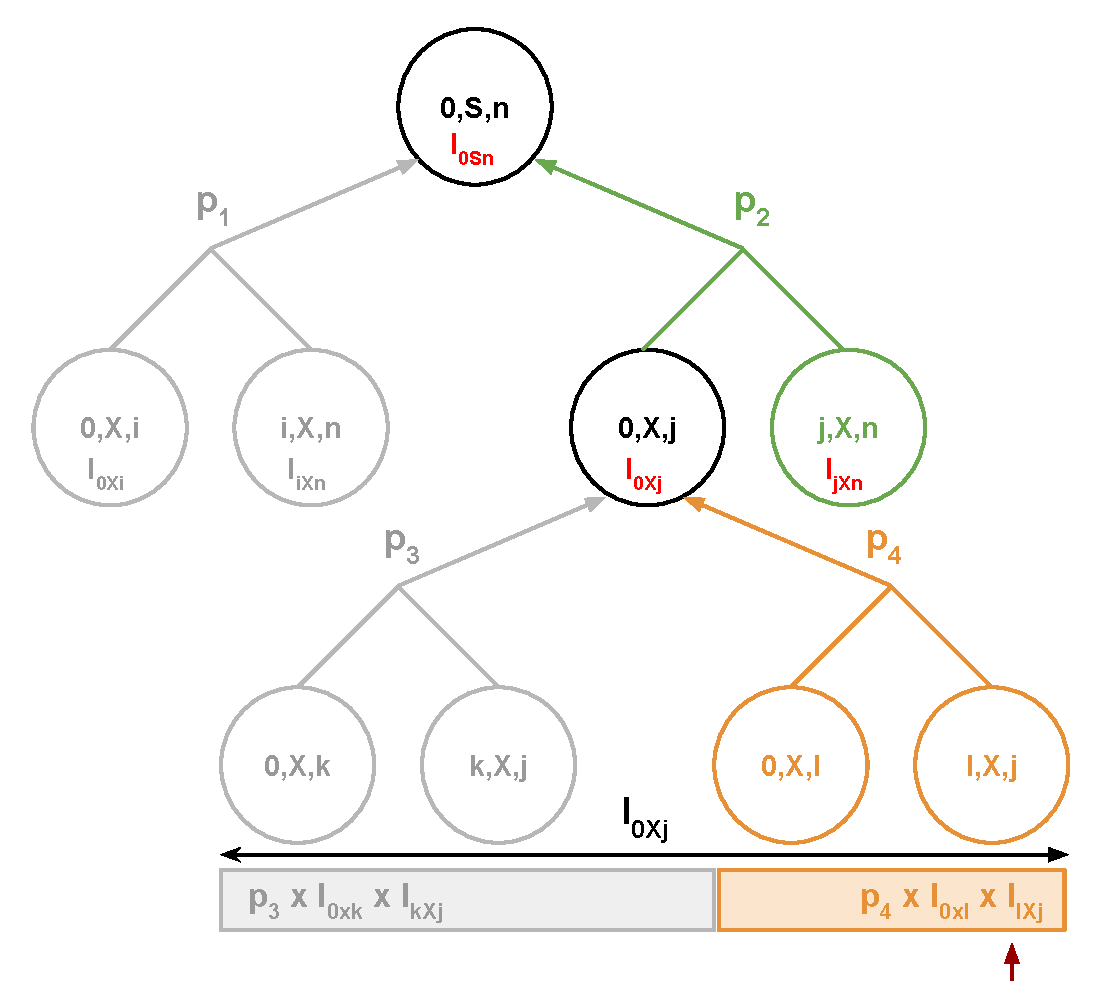
\includegraphics[scale=0.3]{img/sampling10}
	}



}

\frame{
	\frametitle{An example for hierarchical models}
	
	Model $f(\mdd) = \sum_i \varphi(e_i)$\\
	~ where $\varphi(e_i)$ is a weighted combination of local features
	
	~
	
	Grammar \\
	\begin{center}
	\begin{tabular}{l}
	\cellcolor{blue!20} {$X \ra \angbrack{\ftext{a}, \etext{the}}$} \\
	\cellcolor{green!20} {$X \ra \angbrack{\ftext{luz}, \etext{light}}$} \\
	\cellcolor{yellow!20} {$X \ra \angbrack{\ftext{apague } X_1, \etext{switch } X_1 \etext{ off}}$} \\
	\cellcolor{red!20} {$X \ra \angbrack{X_1 \ftext{ por favor}, \etext{please , } X_1}$} \\
	\cellcolor{black!10} {$X \ra \angbrack{X_1 X_2, X_1, X_2}$} \\
	\cellcolor{black!50} {$S \ra \angbrack{\vdash X_1 \dashv, \vdash X_1 \dashv}$} \\
	\end{tabular}
	\end{center}
	
	~
	
	Input: \ftext{apague a luz por favor} \\
	
	Reference: \etext{please, switch the light off}
}


\frame[plain]{\frametitle{Decoding with local features}
	\begin{adjustwidth}{-2em}{-2em}
	\begin{footnotesize}
	\begin{tabular}{| c | p{1cm}  p{1cm}  p{1.1cm}  p{1cm}  p{1cm} | c |}
	\hline
	\textsc{Node}
	  & \multicolumn{1}{c}{{apague}} 
	  & \multicolumn{1}{c}{{a}} 
	  & \multicolumn{1}{c}{{luz}} 
	  & \multicolumn{1}{c}{{por}} 
	  & \multicolumn{1}{c|}{{favor}}
	  & \textsc{Inside} \\   \hline\hline 

	% ONE
	\only<2->{$X_{1,2}$} &        
	& \only<2->{\cellcolor{blue!20} $e_1: \frac{\ftext{a}}{\etext{the}}$}
	&  
	& 
	& 
	& \only<15->{$w(e_1)$} \\ \hline %\hline

	\only<3->{$X_{2,3}$} &        
	& 
	& \only<3->{\cellcolor{green!20} $e_2: \frac{\ftext{luz}}{\etext{light}}$}
	& 
	& 
	& \only<16->{$w(e_2)$} \\ \hline %\hline
	
	\only<4->{$X_{1,3}$} &        
	& \multicolumn{2}{c}{\only<4->{\cellcolor{black!10} $e_3: \frac{X_{1,2} X_{2,3}}{X_{1,2} X_{2,3}}$}}
	& 
	& 
	& \only<17->{$w(e_3)\beta(X_{1,2})\beta(X_{2,3})$} \\ \hline %\hline
	
	\only<5->{$X_{0,2}$}        
	& \multicolumn{2}{c}{\only<5->{\cellcolor{yellow!20} $e_4: \frac{\ftext{apague } X_{1,2}}{\etext{switch } X_{1,2} \etext{off}}$}}
	&
	& 
	& 
	& \only<18->{$w(e_4)\beta(X_{1,2})$} \\ \hline %\hline	

	\only<6->{$X_{2,5}$}        
	& 
	&
	& \multicolumn{3}{c|}{\only<6->{\cellcolor{red!20} $e_5: \frac{X_{2,3} \ftext{ por favor}}{\etext{please, } X_{2,3}}$}}
	&  \only<19->{$w(e_5)\beta(X_{2,3})$} \\ \hline %\hline	

	\multirow{2}{*}{\only<7->{$X_{0,3}$}}
	& \multicolumn{3}{c}{\only<7->{\cellcolor{yellow!20} $e_6: \frac{\ftext{apague } X_{1,3}}{\etext{switch } X_{1,3} \etext{off}}$}}
	&
	& 
	& \only<20->{$w(e_6)\beta(X_{1,3}) \oplus$} \\ %\cline{2-7} %\hline	
	
	%\only<8->{$X_{0,3}$}        
	& \multicolumn{3}{c}{\only<8->{\cellcolor{black!10} $e_7: \frac{X_{0,2} X_{2,3}}{X_{0,2} X_{2,3}}$}}
	&
	& 
	& \only<20->{$w(e_7)\beta(X_{0,2})\beta(X_{2,3})$} \\ \hline
	
	\multirow{2}{*}{\only<9->{$X_{1,5}$}}
	& 
	& \multicolumn{4}{c|}{\only<9->{\cellcolor{red!20} $e_8: \frac{X_{1,3} \ftext{ por favor}}{\etext{please, } X_{1,3}}$}} 
	& \only<21->{$w(e_8)\beta(X_{1,3}) \oplus$} \\ %\cline{2-7} %\hline	
	
	%\multirow{2}{*}{\only<9->{$X_{1,5}$}}
	& 
	& \multicolumn{4}{c|}{\only<10->{\cellcolor{black!10} $e_{9}: \frac{X_{1,2} X_{2,5}}{X_{1,2} X_{2,5}}$}} 
	& \only<21->{$w(e_{9})\beta(X_{1,2})\beta(X_{2,5})$} \\ \hline	
	
	\multirow{3}{*}{\only<11->{$X_{0,5}$}}
	& \multicolumn{5}{c|}{\only<11->{\cellcolor{black!10} $e_{10}: \frac{X_{0,2} X_{2,5}}{X_{0,2} X_{2,5}}$}} 
	& \only<22->{$w(e_{10})\beta(X_{0,2})\beta(X_{2,5}) \oplus$} \\ %\cline{2-7} %\hline	
	
	%\multirow{3}{*}{\only<10->{$X_{0,5}$}}
	& \multicolumn{5}{c|}{\only<12->{\cellcolor{yellow!20} $e_{11}: \frac{\ftext{apague } X_{1,5}}{\etext{switch } X_{1,5} \etext{ off}}$}} 
	& \only<22->{$w(e_{11})\beta(X_{1,5}) \oplus$} \\ %\cline{2-7} %\hline
	
	%\multirow{3}{*}{\only<10->{$X_{0,5}$}}
	& \multicolumn{5}{c|}{\only<13->{\cellcolor{red!20} $e_{12}: \frac{X_{0,3} \ftext{ por favor}}{\etext{please, } X_{0,3}}$}} 
	& \only<22->{$w(e_{12})\beta(X_{0,3})$} \\ \hline
	
	\only<14->{$S_{0,5}$}
	& \multicolumn{5}{c|}{\only<14->{\cellcolor{black!50} $e_{13}: \frac{\vdash X_{0,5} \dashv}{\vdash X_{0,5} \dashv}$}} 
	& \only<23->{$w(e_{13})\beta(X_{0,5})$} \\ \hline

	\end{tabular}
	\end{footnotesize}
	\end{adjustwidth}
}



\frame{
	\frametitle{The problem}
	
	Most interesting models employ nonlocal features!
	
	\begin{itemize}
		\item reordering model: previously translated span
		\item language model: generated strings
	\end{itemize}\pause
	
	Example
	
	$$f(\mdd) = \psi(\yield(\mdd)) + \sum_i \varphi(e_i)$$
	
	~ where $\psi(\myy) = w_\psi \log p_{\textsc{LM}}(\myy)$\\
	~ and $p_{\textsc{LM}}(\myy) = \prod_i p(y_i|y_{i - n + 1}^{i-1})$ is an $n$-gram LM

	\pause
	\begin{itemize}
		\item $p_{\textsc{LM}}$ violates independence assumptions
	\end{itemize}
	
}

\frame{
	\frametitle{Illustration of the problem}
	
	\begin{columns}
		\begin{column}{0.4\textwidth}
			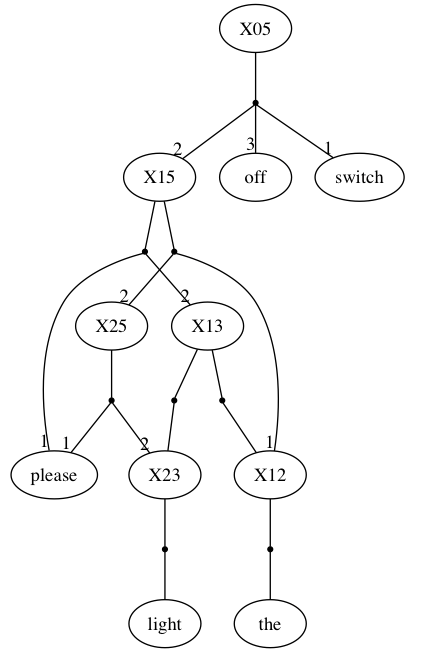
\includegraphics[scale=0.3]{img/switchoff}
		\end{column}
		\begin{column}{0.6\textwidth}
			How do we score the top edge?
			\begin{itemize}
				\item $[\text{switch } [\text{please } [[\text{the}] [\text{light}]]] \text{ off}]$
				\item $[\text{switch } [[\text{the}] [\text{please }[\text{light}]]] \text{ off}]$
			\end{itemize}
		\end{column}

	\end{columns}
}

\frame{
	\frametitle{The solution}
	
	``Hard-code'' structural dependencies
	\begin{itemize}
		\item disambiguate nodes w.r.t. the context they offer to feature functions 
		\item intuition: we will be ``splitting'' nodes
		\item more intuition: nodes must memorise how to complete boundary $n$-grams 
	\end{itemize}
	

}

\frame{
	\frametitle{The intuition}
	
	\begin{columns}
		\begin{column}{0.4\textwidth}
			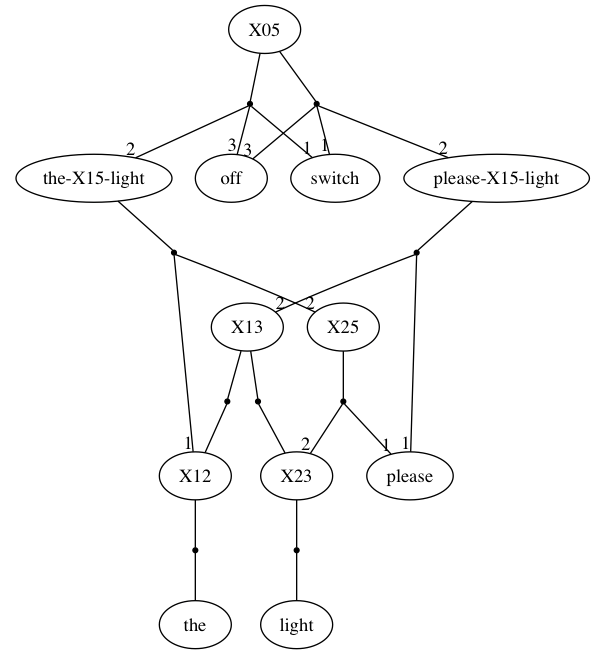
\includegraphics[scale=0.3]{img/switchoff2}
		\end{column}
		\begin{column}{0.6\textwidth}

			\begin{itemize}
				\item hard-code dependencies through nonterminals
				\item now we can weight edges independently even with a bigram LM
			\end{itemize}
		\end{column}

	\end{columns}

}



\frame{
	\frametitle{An example for hierarchical models}
	
	Model $f(\mdd) = \psi(\yield(\mdd)) \sum_i \varphi(e_i)$ \\
	~ where $\varphi(e_i)$ is a weighted combination of local features \\
	~ $\psi(\yield(\mdd))$ contains a $3$-gram LM\\
	~ i.e, $p_{\textsc{LM}_3}(\myy) = \prod_i p(y_i|y_{i-2} y_{i-1})$
	
	~
	
	Grammar \\
	\begin{center}
	\begin{tabular}{l}
	\cellcolor{blue!20} {$X \ra \angbrack{\ftext{a}, \etext{the}}$} \\
	\cellcolor{green!20} {$X \ra \angbrack{\ftext{luz}, \etext{light}}$} \\
	\cellcolor{yellow!20} {$X \ra \angbrack{\ftext{apague } X_1, \etext{switch } X_1 \etext{ off}}$} \\
	\cellcolor{red!20} {$X \ra \angbrack{X_1 \ftext{ por favor}, \etext{please , } X_1}$} \\
	\cellcolor{black!10} {$X \ra \angbrack{X_1 X_2, X_1, X_2}$} \\
	\cellcolor{black!50} {$S \ra \angbrack{\vdash X_1 \dashv, \vdash X_1 \dashv}$} \\
	\end{tabular}
	\end{center}
	
	~
	
	Input: \ftext{apague a luz por favor} \\
	
	Reference: \etext{please, switch the light off}
}




\frame[plain]{%\frametitle{Decoding with a $3$-gram LM}
\begin{adjustwidth}{-2.5em}{-2.5em}
	\begin{footnotesize}
	\begin{tabular}{|>{\scriptsize} p{0.5cm} | p{1cm}  p{1cm}  p{1.1cm}  p{1cm}  p{1cm} |>{\tiny} p{1.5cm} |>{\tiny} p{1cm} |>{\scriptsize} c | }
	\hline
	  & \multicolumn{1}{c}{{apague}} 
	  & \multicolumn{1}{c}{{a}} 
	  & \multicolumn{1}{c}{{luz}} 
	  & \multicolumn{1}{c}{{por}} 
	  & \multicolumn{1}{c|}{{favor}}
	  & {\footnotesize \textsc{Left}} & {\footnotesize \textsc{Right}} & \textsc{Node} \\   \hline\hline 

	% ONE
	\only<2->{$X_{1,2}$} &        
	& \only<2->{\cellcolor{blue!20} $e_1: \frac{\ftext{a}}{\etext{the}}$}
	&  
	& 
	& 
	& \only<2->{the} & \only<2->{the} & 1 \\ \hline %\hline

	\only<3->{$X_{2,3}$} &        
	& 
	& \only<3->{\cellcolor{green!20} $e_2: \frac{\ftext{luz}}{\etext{light}}$}
	& 
	& 
	& \only<3->{light} & \only<3->{light} & 2 \\ \hline %\hline
	
	\only<4->{$X_{1,3}$} &        
	& \multicolumn{2}{c}{\only<4->{\cellcolor{black!10} $e_3: \frac{X_{1,2} X_{2,3}}{(1) ~ (2)}$}}
	& 
	& 
	& \only<4->{the light} & \only<4->{the light} & 3 \\ \hline %\hline
	
	\only<5->{$X_{0,2}$}        
	& \multicolumn{2}{c}{\only<5->{\cellcolor{yellow!20} $e_4: \frac{\ftext{apague } X_{1,2}}{\etext{switch } (1) \etext{ off}}$}}
	&
	& 
	& 
	& \only<5->{switch the} & \only<5->{the off} & 4 \\ \hline %\hline	

	\only<6->{$X_{2,5}$}        
	& 
	&
	& \multicolumn{3}{c|}{\only<6->{\cellcolor{red!20} $e_5: \frac{X_{2,3} \ftext{ por favor}}{\etext{please, } (2)}$}}
	& \only<6->{please ,} & \only<6->{, light} & 5 \\ \hline %\hline	

	\multirow{2}{*}{\only<7->{$X_{0,3}$}}
	& \multicolumn{3}{c}{\only<7->{\cellcolor{yellow!20} $e_6: \frac{\ftext{apague } X_{1,3}}{\etext{switch } (3) \etext{ off}}$}}
	&
	& 
	& \only<7->{switch the} & \only<7->{light off} & 6  \\ \cline{2-9} 
	
	%\only<8->{$X_{0,3}$}        
	& \multicolumn{3}{c}{\only<8->{\cellcolor{black!10} $e_7: \frac{X_{0,2} X_{2,3}}{(4) ~ (2)}$}}
	&
	& 
	&  \only<8->{switch the} & \only<8->{off light} & 7  \\ \hline
	
	\multirow{2}{*}{\only<9->{$X_{1,5}$}}
	& 
	& \multicolumn{4}{c|}{\only<9->{\cellcolor{red!20} $e_8: \frac{X_{1,3} \ftext{ por favor}}{\etext{please, } (3)}$}} 
	&  \only<9->{please ,} & \only<9->{the light} & 8 \\ \cline{2-9} %\hline	
	
	%\multirow{2}{*}{\only<9->{$X_{1,5}$}}
	& 
	& \multicolumn{4}{c|}{\only<10->{\cellcolor{black!10} $e_9: \frac{X_{1,2} X_{2,5}}{(1) ~ (5)}$}} 
	& \only<10->{the please} & \only<10->{, light} & 9 \\ \hline	
	
	\multirow{4}{*}{\only<11->{$X_{0,5}$}}
	& \multicolumn{5}{c|}{\only<11->{\cellcolor{black!10} $e_{10}: \frac{X_{0,2} X_{2,5}}{(4) ~ (5)}$}} 
	& \only<11->{switch the} & \only<11->{, light} & 10 \\ \cline{2-9} \cline{2-8}	
	
	%\multirow{3}{*}{\only<10->{$X_{0,5}$}}
	& \multicolumn{5}{c|}{\only<12->{\cellcolor{yellow!20} $e_{11}: \frac{\ftext{apague } X_{1,5}}{\etext{switch } (8) \etext{ off}}$}} 
	& \only<12->{switch please} & \only<12->{light off} & 11 \\ \cline{2-9}
	
	%\multirow{3}{*}{\only<10->{$X_{0,5}$}}
	& \multicolumn{5}{c|}{\only<13->{\cellcolor{yellow!30} $e_{12}: \frac{\ftext{apague } X_{1,5}}{\etext{switch } (9) \etext{ off}}$}} 
	& \only<13->{switch the} & \only<13->{light off} & 12 \\ \cline{2-9}
		
	%\multirow{3}{*}{\only<10->{$X_{0,5}$}}
	& \multicolumn{5}{c|}{\only<14->{\cellcolor{red!20} $e_{13}: \frac{X_{0,3} \ftext{ por favor}}{\etext{please, } (6)}$}} 
	&  \only<14->{please ,} & \only<14->{light off} & 13 \\  \cline{2-9}
	
	& \multicolumn{5}{c|}{\only<15->{\cellcolor{red!30} $e_{14}: \frac{X_{0,3} \ftext{ por favor}}{\etext{please, } (7)}$}} 
	&  \only<15->{please ,} & \only<15->{off light} & 14 \\ \hline
	
	\multirow{4}{*}{\only<16->{$S_{0,5}$}}
	& \multicolumn{5}{c|}{\only<16->{\cellcolor{black!40} $e_{15}: \frac{\vdash X_{0,5} \dashv}{\vdash (10) \dashv}$}} 
	& \only<16->{$\vdash$ switch} & \only<16->{light $\dashv$} & 15 \\ \cline{2-9}
	
	& \multicolumn{5}{c|}{\only<17->{\cellcolor{black!45} $e_{16}: \frac{\vdash X_{0,5} \dashv}{\vdash (11) \dashv}$}
	\only<18->{\cellcolor{black!45} or $e_{17}: \frac{\vdash X_{0,5} \dashv}{\vdash (12) \dashv}$}
	} 
	& \only<17->{$\vdash$ switch} & \only<17->{off $\dashv$} & 16 \\ \cline{2-9}
	
	& \multicolumn{5}{c|}{\only<19->{\cellcolor{black!50} $e_{18}: \frac{\vdash X_{0,5} \dashv}{\vdash (13) \dashv}$}} 
	& \only<19->{$\vdash$ please} & \only<19->{off $\dashv$} & 17 \\ \cline{2-9}
	
	& \multicolumn{5}{c|}{\only<20->{\cellcolor{black!55} $e_{19}: \frac{\vdash X_{0,5} \dashv}{\vdash (14) \dashv}$}} 
	& \only<20->{$\vdash$ please} & \only<20->{light $\dashv$} & 18 \\ \hline

	\end{tabular}
	\end{footnotesize}
\end{adjustwidth}
}


\frame{
	\frametitle{The problem with the solution}

	\pause
	
	Computational complexity!
	
	\pause
	\begin{enumerate}
		\item it seems like the underlying grammar is growing
		\item there are way too many $n$-grams leading to way too many nonterminals 
		\item the graphical representation (forest) is growing
	\end{enumerate}
	

	
}

\frame{
	\frametitle{What is really going on?}
	
	We are transferring memory from an automaton to the forest \pause
	\begin{itemize}
		\item $n$-gram LMs can be thought of as an automaton\\
		where each state $q$ uniquely represents a $k$-gram prefix $\alpha_q$  $(k < n)$\\ \pause
		\item a transition from a state $q$ labelled with word $w$ is weighted by the probability $p(w|\alpha_q)$
	\end{itemize}
	
	\pause
	
	A nonterminal in the forest yields a set of strings \pause
	\begin{itemize}
		\item strings project onto paths in the LM automaton \pause
		\item paths are weighted
	\end{itemize}
	\pause
	
	Nonterminals must be aware of (parts of) the strings they yield \pause
	\begin{itemize}
		\item they must be annotated with states of the automaton
	\end{itemize}
	
}

\frame{
	\frametitle{How hard is it?}
	
	Weighted intersection between a wCFG and a wFSA \pause
	
	~
	
	Generalisation of parsing for \pause
	\begin{itemize}
		\item arbitrary automata \pause
		\item weighted sets
	\end{itemize}
	
	~\pause
	
	Complexity\pause
	\begin{itemize} 
		\item input: $X_0 \ra X_1 X_2 \ldots X_{a}$ where $X_i \in N$ \pause
		\item output: $X_0^{(q_1, q_a)} \ra X_1^{(q_1, q_2)} X_2^{(q_2, q_3)} \ldots X_{a}^{(q_{a-1}, q_a)}$  \\ where $q_j \in Q$ \pause
		\item complexity: $O(|N||Q|^{a + 1})$
	\end{itemize}
}

\frame{
	\frametitle{Solution}

	The usual suspect
	\begin{itemize}
		\item pruning
	\end{itemize}
	
	~
	
	\pause
	Alternatives
	\begin{itemize}
		\item local search (greedy methods)
		\item relaxation techniques 
		\item sampling 
	\end{itemize}
}

\frame{
	\frametitle{Pruning: beam search}
	
	Approximate intersection by	budgeting the combination of ``comparable'' nodes \pause

	\begin{itemize}
		\item nodes that share structure \pause
		\begin{itemize}
			\item phrase-based: coverage vector
			\item hierarchical: input spans
		\end{itemize}\pause
		\item heuristic view of interaction with LM
		\begin{itemize}
			\item phrase-based: approximate future cost  
			\item local approximation based on limited context
		\end{itemize}
	\end{itemize}
}

\frame{
	\frametitle{Naive beam search}
	\only<1>{
	\begin{enumerate}
		\item enumerate combinations
		\item sort and prune all but the $k$ best
	\end{enumerate}
	}
	\only<2>{
	\begin{center}
		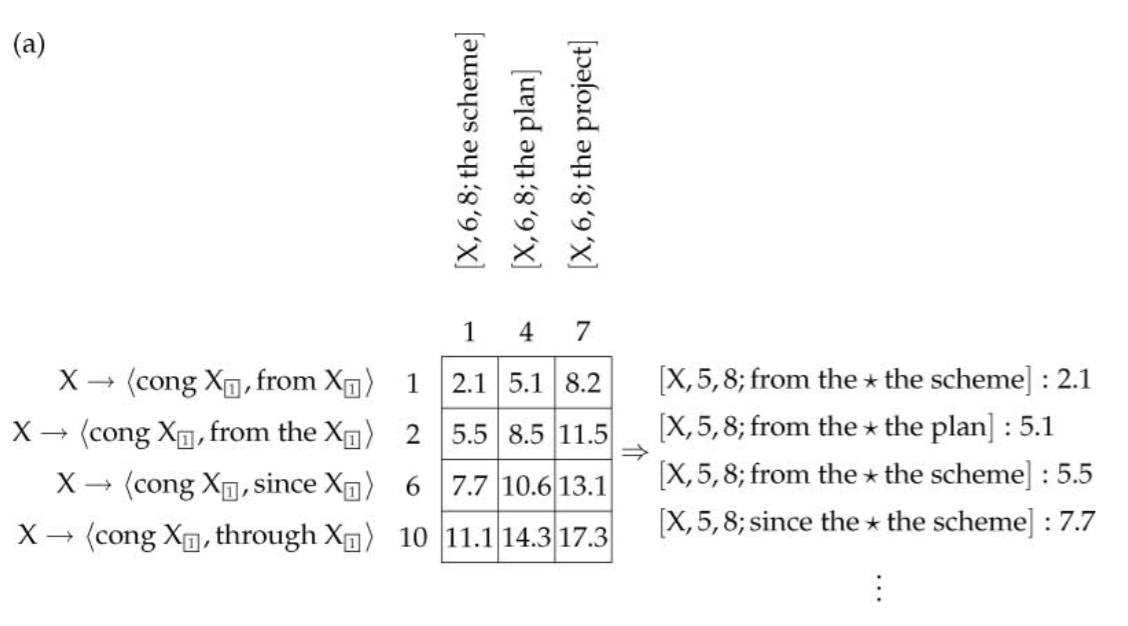
\includegraphics[scale=0.3]{img/beamsearch}
	\end{center}
	}
}

\frame{
	\frametitle{Cube pruning}
	
	\only<1>{
	An agenda for pruning \citep{Chiang:2007:HPT}
	\begin{itemize}
		\item tries to enumerate combinations in best-first order
		\item stops after $k$ items have been enumerated
		\item inspiration: product of sorted lists
		\item heuristic: assumes the LM a monotone function over edges
	\end{itemize}
	}
	\only<2>{
	\begin{center}
		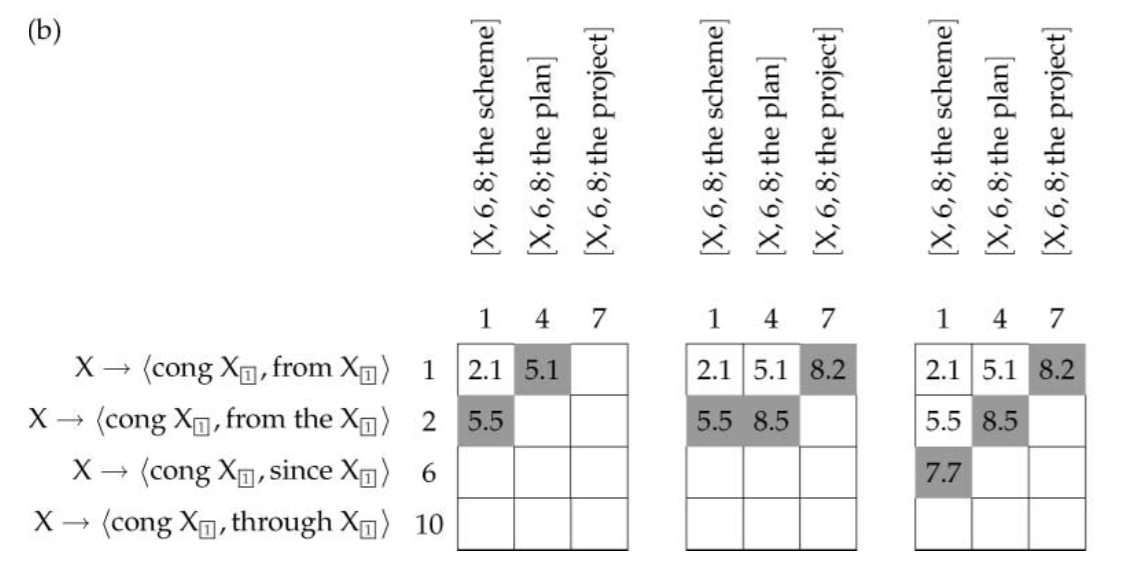
\includegraphics[scale=0.3]{img/cubepruning}
	\end{center}
	}
}

\frame{
	\frametitle{Problem with pruning}
	
	\begin{enumerate}
		\item unbounded approximation
		\item approximating the Viterbi solution
		\item incompatible with models which have a probabilistic interpretation
		\item cannot handle arbitrarily nonlocal dependencies
	\end{enumerate}
}

\frame{
	\frametitle{Beyond beam search}
	
	Local search \citep{Hardmeier+2012:DocDec}
	\begin{itemize}
		\item computationally cheap
		\item unbounded approximation
		\item approximate Viterbi
		\item can handle arbitrarily nonlocal dependencies
		\item too local view of the distribution (bad for tuning)
	\end{itemize}
	
}

\frame{
	\frametitle{Beyond beam search}
	
	Relaxation methods \\
	\citep{Chang+2011:pbsmt,Rush+2011:hpbsmt}
	\begin{itemize}
		\item computationally expensive
		\item bounded approximation
		\item (approximate) Viterbi
		\item may handle arbitrarily nonlocal dependencies
	\end{itemize}
	
}

\frame{
	\frametitle{Beyond beam search}
	
	Sampling \citep{Arun+2009:MC,Aziz+2013:osstar,Aziz:2014:phd}
	\begin{itemize}
		\item (bounded) approximation
		\item (approximate) Viterbi, expectations
		\item handle arbitrarily nonlocal dependencies
		\item in principle ideal for tuning (global view of distribution)
		\item potentially computationally expensive
	\end{itemize}
	
}